% Asset ID: A21BinomialExpansionTikZ-006
% Unit: A21
% Topic code: A21-SS
% Topic ID: A21BinomialExpansion
% Purpose: Approximation workflow
\documentclass[tikz,border=10pt]{standalone}
\usepackage{amsmath}
\usetikzlibrary{arrows.meta,positioning}
\begin{document}
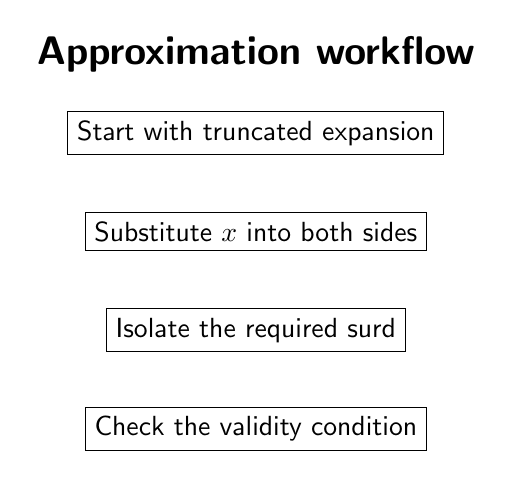
\begin{tikzpicture}[every node/.style={font=\sffamily}]
\node[font=\sffamily\bfseries\Large] at (0,3) {Approximation workflow};
\node[draw,align=center] at (0,2) {Start with truncated expansion};\node[draw,align=center] at (0,0.75) {Substitute $x$ into both sides};\node[draw,align=center] at (0,-0.5) {Isolate the required surd};\node[draw,align=center] at (0,-1.75) {Check the validity condition};
\end{tikzpicture}
\end{document}
